\documentclass[12pt]{article}
\usepackage[utf8]{inputenc}
\usepackage{amsmath}
\usepackage{amsfonts}
\usepackage{amssymb}
\usepackage{empheq}
\usepackage{tikz}
\usepackage{enumitem}
\usepackage{eucal}
\usepackage{changepage}
\usetikzlibrary{automata, positioning, shapes, decorations.markings}
\addtolength{\topmargin}{-0.75in}
\addtolength{\textheight}{1.75in}
\addtolength{\evensidemargin}{-0.5in}

\title{Topology Homework 07}
\author{Ethan Jensen}
\date{March 18, 2020}

\begin{document}
  \maketitle
  \noindent
  \textbf{EXERCISE 3.23}
  If \(\mathbb{R}\) has the standard topology, define
  \[p:\mathbb{R}\rightarrow \{a,b,c,d,e\} \textup{ by } p(x) = \left\{\begin{array}{ccc}
  a \textup{ if } x > 2 \ \ \ \ \ \ \ \ \ \\
  b \textup{ if } x = 2 \ \ \ \ \ \ \ \ \ \\
  c \textup{ if } 0 \leq x < 2 \ \ \ \ \\
  d \textup{ if } -1 < x < 0 \\
  e \textup{ if } x \leq -1 \ \ \ \ \ \ \
  \end{array}\right.\]
  \textbf{(a)}\ List the open sets in the quotient topology on \(\{a,b,c,d,e\}\).
  \newline
  \textbf{(b)}\ Now assume that \(\mathbb{R}\) has the lower limit topology. What are the open sets in the resulting quotent topology on \(\{a,b,c,d,e\}\)?
  \newline \newline
  The collection of open sets \(\mathcal{T}\) assuming the standard topology is
  \[\mathcal{T} = \{\{a\},\{d\},\{a,d\},\{c,d\},\{d,e\},\{a,c,d\},\]
  \[\{a,d,e\},\{c,d,e\},\{a,c,d,e\},\{a,b,c,d\},\{a,b,c,d,e\},\varnothing\}\]
  \newline
  The collection of open sets \(\mathcal{T}\) assuming the lower limit topology is
  \[\mathcal{T} = \{\{a\},\{c\},\{d\},\{a,d\},\{a,b\},\{a,c\},\{c,d\},\{d,e\},\{a,b,c\},\{a,b,d\},\{a,c,d\},\]
  \[\{a,d,e\},\{c,d,e\},\{a,b,c,d\},\{a,b,d,e\},\{a,c,d,e\},\{a,b,c,d\},\{a,b,c,d,e\},\varnothing\}\]
  \newpage
  \noindent
  \textbf{EXERCISE 2.24}
  Let \(X = \mathbb{R}\) in the standard topology. Take the partition
  \[X^*=\{...(-1,0],(0,1],(1,2],...\}.\]
  Describe the open sets in the resulting quotient topology on \(X^*\).
  \newline \newline
  None of the open sets in \(X^*\) are open in the standard topology on \(\mathbb{R}\).
  \newline
  Thus, the resulting quotient topology on \(X^*\) is the trivial topology:
  \[\mathcal{T} = \{\varnothing, X\}\]
  \newpage
  \noindent
  \textbf{EXERCISE 2.25}
  Define a partition of \(X = \mathbb{R^2} - \{O\}\) by taking each ray emanating from the origin as an element in the partition. Which topological space that we have previously encountered appears to be topologically equivalent to the quotient space that results from this partition?
  \newline
  \newline
  The subspace topology of \(\mathbb{R}^2\) onto the circle \(S_1\) appears to be topologically equivalent.
  \newpage
  \noindent
  \textbf{EXERCISE 2.26}
  Devise the rules for a game of tic-tac-toe that is played on the surface of the torus, using the square model of the torus as illustrated in Figure 1. What new three-in-a-rows would this game allow that are not allowed in the standard game?
  \newline
  \begin{figure}[ht]
    \centering
    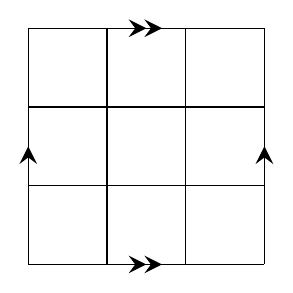
\begin{tikzpicture}[arrow inside/.style =
         {
             postaction={decorate},
             decoration={markings, mark=at position 0.5 with {\arrow[scale = 2,>=stealth]{>}}}
         }]
      \draw
      (0,1) edge[]  (3,1)
      (0,2) edge[]  (3,2)
      (1,0) edge[]  (1,3)
      (2,0) edge[]  (2,3);

      \draw[arrow inside] (0.4,0) --  (3,0);
      \draw[arrow inside] (0.4,3) --  (3,3);
      \draw[arrow inside] (0,0) --  (3,0);
      \draw[arrow inside] (0,3) --  (3,3);
      \draw[arrow inside] (0,0) --  (0,3);
      \draw[arrow inside] (3,0) --  (3,3);
    \end{tikzpicture}
    \caption{Tic-tac-toe on a torus}
  \end{figure}
  \newline
  \begin{figure}[ht]
    \centering
    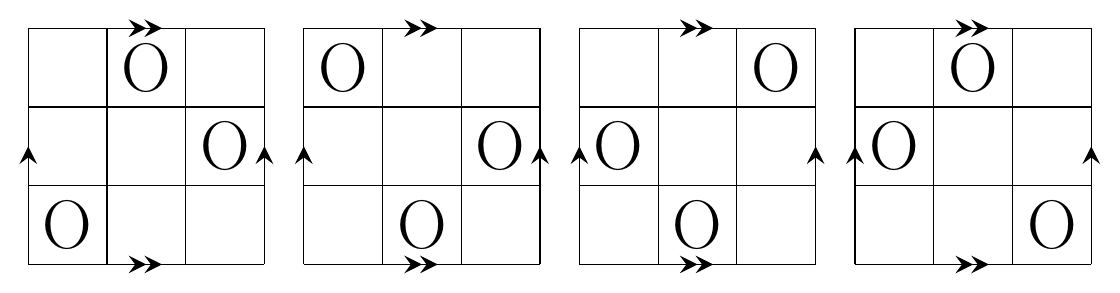
\begin{tikzpicture}[arrow inside/.style =
         {
             postaction={decorate},
             decoration={markings, mark=at position 0.5 with {\arrow[scale = 2,>=stealth]{>}}}
         }]
      \draw
      (-3.5,1) edge[]  (-0.5,1)
      (-3.5,2) edge[]  (-0.5,2)
      (-2.5,0) edge[]  (-2.5,3)
      (-1.5,0) edge[]  (-1.5,3);

      \draw[arrow inside] (-3.1,0) --  (-0.5,0);
      \draw[arrow inside] (-3.1,3) --  (-0.5,3);
      \draw[arrow inside] (-3.5,0) --  (-0.5,0);
      \draw[arrow inside] (-3.5,3) --  (-0.5,3);
      \draw[arrow inside] (-3.5,0) --  (-3.5,3);
      \draw[arrow inside] (-0.5,0) --  (-0.5,3);

      \draw
      (0,1) edge[]  (3,1)
      (0,2) edge[]  (3,2)
      (1,0) edge[]  (1,3)
      (2,0) edge[]  (2,3);

      \draw[arrow inside] (0.4,0) --  (3,0);
      \draw[arrow inside] (0.4,3) --  (3,3);
      \draw[arrow inside] (0,0) --  (3,0);
      \draw[arrow inside] (0,3) --  (3,3);
      \draw[arrow inside] (0,0) --  (0,3);
      \draw[arrow inside] (3,0) --  (3,3);

      \draw
      (3.5,1) edge[]  (6.5,1)
      (3.5,2) edge[]  (6.5,2)
      (4.5,0) edge[]  (4.5,3)
      (5.5,0) edge[]  (5.5,3);

      \draw[arrow inside] (3.9,0) --  (6.5,0);
      \draw[arrow inside] (3.9,3) --  (6.5,3);
      \draw[arrow inside] (3.5,0) --  (6.5,0);
      \draw[arrow inside] (3.5,3) --  (6.5,3);
      \draw[arrow inside] (3.5,0) --  (3.5,3);
      \draw[arrow inside] (6.5,0) --  (6.5,3);

      \draw
      (7,1) edge[]  (10,1)
      (7,2) edge[]  (10,2)
      (8,0) edge[]  (8,3)
      (9,0) edge[]  (9,3);

      \draw[arrow inside] (7.4,0) --  (10,0);
      \draw[arrow inside] (7.4,3) --  (10,3);
      \draw[arrow inside] (7,0) --  (10,0);
      \draw[arrow inside] (7,3) --  (10,3);
      \draw[arrow inside] (7,0) --  (7,3);
      \draw[arrow inside] (10,0) --  (10,3);

      \node[] (s0) at (-2,2.5) {\Huge{O}};
      \node[] (s1) at (-1,1.5) {\Huge{O}};
      \node[] (s2) at (-3,0.5) {\Huge{O}};

      \node[] (s0) at (0.5,2.5) {\Huge{O}};
      \node[] (s1) at (2.5,1.5) {\Huge{O}};
      \node[] (s2) at (1.5,0.5) {\Huge{O}};

      \node[] (s0) at (6,2.5) {\Huge{O}};
      \node[] (s1) at (4,1.5) {\Huge{O}};
      \node[] (s2) at (5,0.5) {\Huge{O}};

      \node[] (s0) at (8.5,2.5) {\Huge{O}};
      \node[] (s1) at (7.5,1.5) {\Huge{O}};
      \node[] (s2) at (9.5,0.5) {\Huge{O}};
    \end{tikzpicture}
  \end{figure}
  \newpage
  \noindent
  \textbf{EXERCISE 3.27}
  Provide an example showing that a quotient space of a Hausdorff space need not be a Hausdorff space.
  \newline \newline
  Consider \(\mathbb{R}\) with the standard topology.
  \newline
  We have shown that \(\mathbb{R}\) is Hausdorff in a previous exercise.
  \newline \newline
  Consider the following surjective function \(p:\mathbb{R}\rightarrow \mathbb{Z}\) defined by
  \[p(x) = \left\{\begin{array}{ccc}
  x \textup{ if } x \in \mathbb{Z} \ \ \ \ \ \ \ \ \ \ \ \ \ \ \ \ \ \ \ \ \ \ \ \ \ \ \ \ \ \ \ \ \ \\
  n \textup{ if } x \in (n-1, n+1) \textup{ and n is odd}
  \end{array}\right.\]
  \newline
  The quotient space of the standard topology on \(\mathbb{R}\) defined by p is the digital line topology on \(\mathbb{Z}\).
  \newline \newline
  It is easy to see that the basis for that topology defined by p is \[\mathbb{B}=\{\{2n+1\},\{2n-1, 2n, 2n+1\}|\ n \in \mathbb{Z}_+\}\]
  Every open set in a topology can be written as a union of basis elements. There is only one basis element that contains the point 2 - which is \(\{1,2,3\}\).
  \newline \newline
  Thus, every open neighborhood of the point 2 also contains the point 3.
  \newline
  So the digital line topology on \(\mathbb{Z}\) is not Hausdorff.
  \newline \(\square\)
  \newpage
  \noindent
  \textbf{EXERCISE 3.28}
  Consider the equivalence relation on \(\mathbb{R}\) defined by \(x ~ y\) if \(x - y \in \mathbb{Z}\). Describe the quotient space that results from the partition of \(\mathbb{R}\) into the equivalence classes in the equivalence relation.
  \newline \newline
  We generate the quotient topology from the subspace topology of \(\mathbb{R}^2\) on \(S_1\) to \([0,1)\) defined by p where
  \newline
  \(p:S_1 \rightarrow [0,1)\) is defined by
  \[p(x,y) = \frac{1}{2\pi}\tan^{-1}\left(\frac{y}{x}\right)\].
  \newline
  Call the quotient space that results from the partition of \(\mathbb{R}\) into the equivalence classes in the equivalence relation \(\mathbb{R}_q\)
  \newline \newline
  V is open in \(\mathbb{R}_q\) iff \(\mathbb{R}_q = \bigcup_{i=1}^{\infty}U_i\)
  where \(U_i = \{x+i|\ x \in U, \textup{U is open in [0,1)}\}\)
  \newline \newline
  In words, it takes open sets on \([0,1)\), and copies them every 1 unit, unioning them together to make an open set in the equivalence relation topology.
  \newpage
  \noindent
  \textbf{EXERCISE 3.33}
  In each of the following cases, describe or draw a picture of the resulting quotient space. Assume that the points are identified only with themselves unless they are explicitly said to be identified with other points.
  \newline
  \textbf{(a)} The disk with its boundary points identified with each other to form a single point. \newline
  \textbf{(b)} The circle \(S^1\) with each pair of antipodal points identified with each other. \newline
  \textbf{(c)} The interval [0,4], as a subspace of \(\mathbb{R}\), with integer points identified with each other. \newline
  \textbf{(d)} The interval [0,9], as a subspace of \(\mathbb{R}\), with even integer points identified with each other to form a point and with odd integers identified with each other to form a different point. \newline
  \textbf{(e)} The real line \(\mathbb{R}\) with [-1,1] collapsed to a point. \newline
  \textbf{(f)} The real line \(\mathbb{R}\) with \([-2,-2] \cup [1,2]\) collapsed to a point. \newline
  \textbf{(g)} The real line \(\mathbb{R}\) with (-1,1) collpased to a point. \newline
  \textbf{(h)} The plane \(\mathbb{R}^2\) with the circle \(S^1\) collapsed to a point. \newline
  \textbf{(i)} The plane \(\mathbb{R}^2\) with the circle \(S^1\) and the origin collapsed to a point. \newline
  \textbf{(j)} The sphere with the north and south pole identified with each other. \newline
  \textbf{(k)} The sphere with the equator collapsed to a point
  \newline
  \newline
  \textit{Drawings on the following page...}
  \newpage
  \includegraphics{IMG318_2}
\end{document}
